\documentclass[11pt]{article}
\usepackage[margin=1in]{geometry}
\usepackage{amsmath,amssymb}
\usepackage{graphicx}
\usepackage{verbatim}
\usepackage{xcolor}
\usepackage[colorlinks=true,linkcolor=blue,urlcolor=blue]{hyperref}
\usepackage{float}

% Numbers produced by assignment1.ipynb (re-run the notebook, then recompile)
\newcommand{\TSN}{212345678}
\newcommand{\xstart}{0.89}
\newcommand{\errA}{1.62\times10^{-4}}
\newcommand{\devX}{1.04\times10^{-3}}
\newcommand{\xmeanEnd}{0.8892}
\newcommand{\normMin}{0.99940}
\newcommand{\Kzero}{0.49991}
\newcommand{\Vzero}{0.52105}
\newcommand{\Kexact}{0.50000}
\newcommand{\Vexact}{0.52105}
\newcommand{\Eexact}{1.02105}
\newcommand{\Emin}{1.01785}
\newcommand{\Emax}{1.02144}
\newcommand{\Edev}{0.31}
\newcommand{\normI}{0.99946}
\newcommand{\normII}{1.1\times10^{258}}
\newcommand{\normIII}{4.1\times10^{51}}
\newcommand{\nFailSix}{372}
\newcommand{\nFailTwelve}{744}


\newcommand{\ev}[1]{\langle #1\rangle}

\title{PHYS 142/242 Assignment 1: Harmonic Oscillator Path Integral}
\author{\textcolor{red}{[Your name]} \quad TSN: \TSN}
\date{}

\begin{document}
\maketitle
\vspace{-1.5em}
\begin{center}
  \fbox{\large $x_{\rm start} = \xstart$}
\end{center}

\noindent
Units: $m=\omega=\hbar=1$, $T_0=2\pi$. Grid: $N_D+1=601$ points on $[-4,4]$, $\Delta x=8/600$; time step $\epsilon=T_0/128$.
All code is in \texttt{assignment1.ipynb}. It writes every figure below, \texttt{animation.gif}, and \texttt{results.json}.
States are evolved as $\psi_{n+1}=\Delta x\,K_\epsilon\,\psi_n$, where $(K_\epsilon)_{ba}=K(x_b,\epsilon;x_a,0)$ is Eq.~(4).
The state is never renormalized.

%--------------------------------------------------------------------
\section*{Problem A: $K_{8\epsilon}$}
Using Eq.~(5) with $N=8$, $K_{8\epsilon}=(\Delta x)^7K_\epsilon^8$ (one factor of $\Delta x$ for each of the 7 intermediate integrals).
Truncated NumPy output (\texttt{print(K\_8eps)}):
{\footnotesize
\verbatiminput{figs/K8eps.txt}}
\noindent
As expected, the matrix is symmetric: $K(x_b,x_a)=K(x_a,x_b)$.
Check: acting on $\psi_0$, $\Delta x\,K_{8\epsilon}\psi_0$ agrees with $\Delta x\,K(8\epsilon)\psi_0$ from Eq.~(4) at $t=8\epsilon$ to a relative error of $\errA$.
Comparing the two matrices element by element is not a meaningful test. A point-source kernel spreads over every $x$ and every momentum, so its entries depend on where the box ends and on the grid's momentum cutoff $\pi/\Delta x$. On a smooth, localized state those effects drop out.

%--------------------------------------------------------------------
\section*{Problem B: $\ev{x}$ over one period}
\begin{figure}[H]
  \centering
  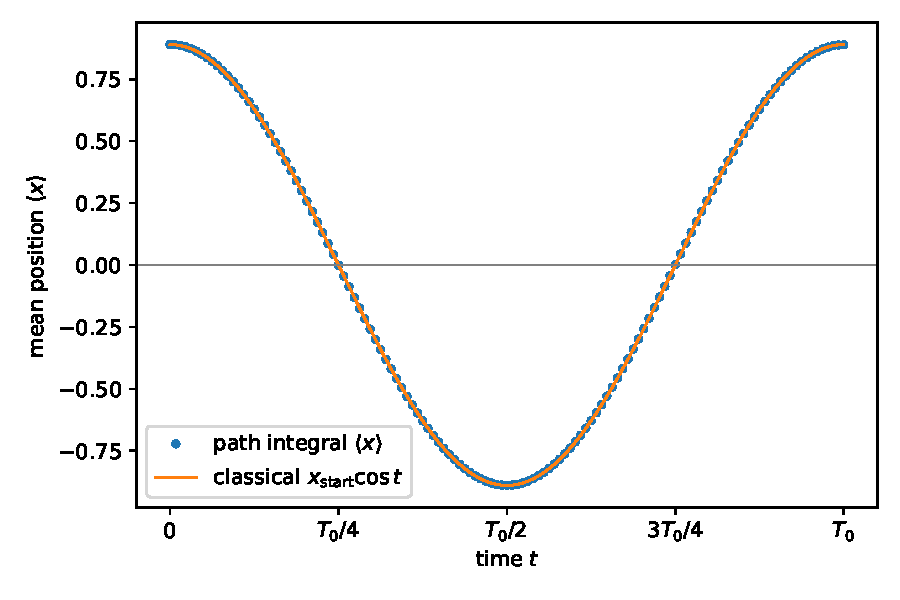
\includegraphics[width=0.62\textwidth]{figs/mean_x.pdf}
  \caption{$\ev{x}=\Delta x\sum_i x_i|\Psi_t(x_i)|^2$ over one period (dots), with the classical trajectory $x_{\rm start}\cos t$ (line).}
\end{figure}
\noindent
As Ehrenfest's theorem requires for a quadratic potential, $\ev{x}$ follows the classical trajectory exactly. The maximum deviation is $\devX$, and after one period $\ev{x}(T_0)=\xmeanEnd$.
The small residual comes from the hard walls at $x=\pm4$. Around $t=T_0/4$ and $3T_0/4$ the packet's tails reach the walls and are cut off. The norm drops to $\normMin$ by $t=T_0$. Repeating the run with walls at $\pm6$ (same $\Delta x$) brings the norm loss down to $\sim3\times10^{-8}$.

%--------------------------------------------------------------------
\section*{Problem C: $\ev{E}$, $\ev{K}$, $\ev{V}$}
\begin{figure}[H]
  \centering
  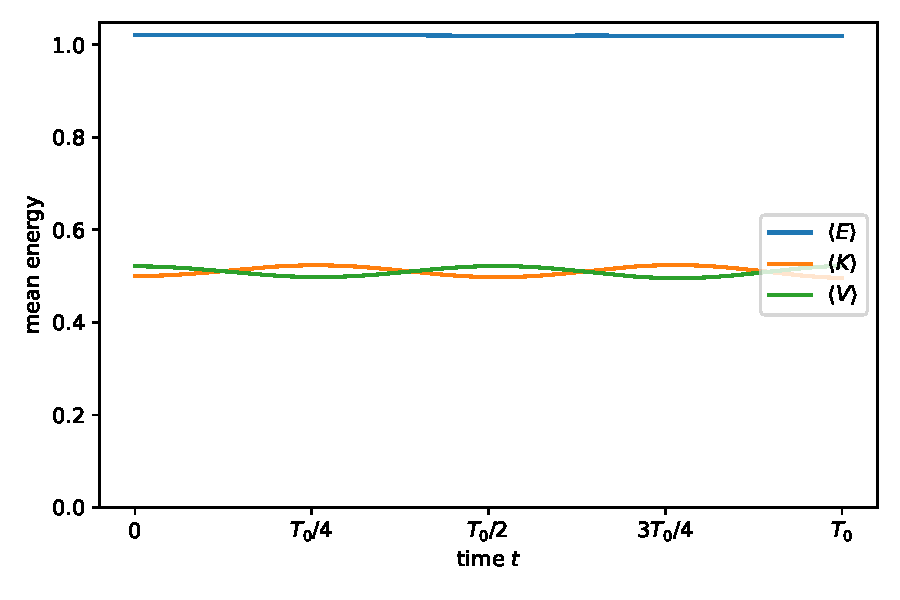
\includegraphics[width=0.62\textwidth]{figs/energy.pdf}
  \caption{Mean total, kinetic, and potential energy over one period. $\ev{V}=\Delta x\sum_i\tfrac12x_i^2P_t(x_i)$ and $\ev{K}=\tfrac12\Delta x\sum_i|\partial_x\Psi_t(x_i)|^2$ (Eq.~8), with the derivative taken by central differences.}
\end{figure}
\noindent
Analytically, the initial Gaussian has $\ev{K}(0)=\alpha/4=\Kexact$ and $\ev{V}(0)=\tfrac12x_{\rm start}^2+\tfrac1{4\alpha}=\Vexact$, so $\ev{E}=\Eexact$.
Numerically, $\ev{K}(0)=\Kzero$ and $\ev{V}(0)=\Vzero$, and $\ev{E}$ stays in $[\Emin,\Emax]$: conserved to $\Edev\%$.
That small drift is again wall leakage: the probability lost near $|x|=4$ carries $V\approx8$ per unit probability. With walls at $\pm6$ the drift drops to $\sim10^{-4}$.

$\ev{K}$ and $\ev{V}$ trade energy back and forth at frequency $2\omega$.
The reason is that $\alpha=2\neq m\omega/\hbar=1$: the initial state is narrower than the ground state (a squeezed state).
The width therefore ``breathes'' twice per period. The position variance is $1/(2\alpha)=0.25$ at $t=0,T_0/2,T_0$ and $\alpha/2=1$ at $t=T_0/4,3T_0/4$ (numerically $0.25$ and $0.996$).
This breathing sits on top of the classical exchange $\tfrac12x_{\rm start}^2\cos^2t \leftrightarrow \tfrac12x_{\rm start}^2\sin^2t$, which also has frequency $2\omega$.

%--------------------------------------------------------------------
\section*{Problem D: amplitudes at $t=mT_0/16$}
\begin{figure}[H]
  \centering
  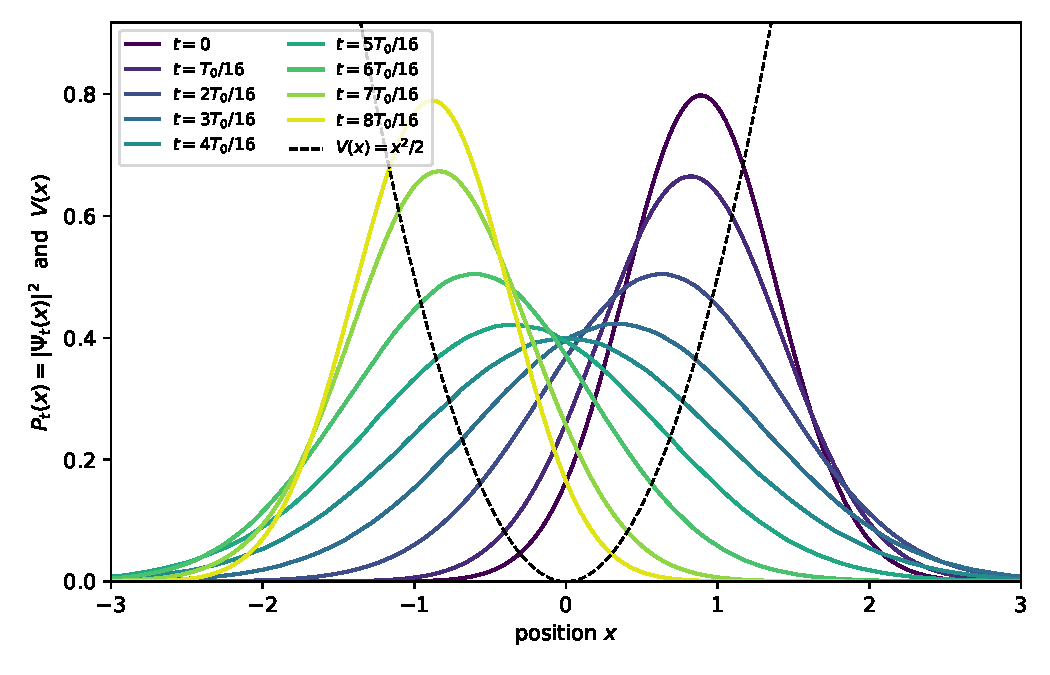
\includegraphics[width=0.49\textwidth]{figs/snapshots.pdf}\hfill
  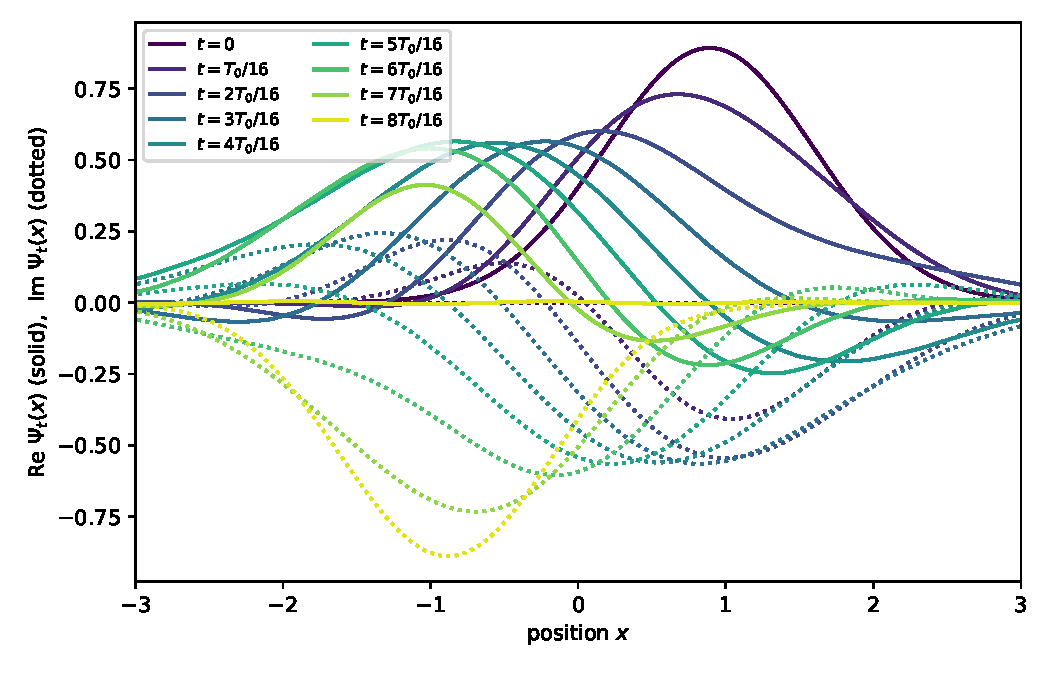
\includegraphics[width=0.49\textwidth]{figs/amplitudes.pdf}
  \caption{Left: $P_t(x)=|\Psi_t(x)|^2$ at $t=mT_0/16$, $m=0,\dots,8$, with $V(x)=x^2/2$ superimposed. Right: $\mathrm{Re}\,\Psi_t$ (solid) and $\mathrm{Im}\,\Psi_t$ (dotted) at the same times.}
\end{figure}
\noindent
Over half a period the packet moves from $x_{\rm start}$ to $-x_{\rm start}$, as in Problem B.
It broadens to its maximum width at $t=T_0/4$ (where it is centered at $x=0$) and then refocuses to its original width at $t=T_0/2$.
In the right panel, the phase develops a linear term $e^{i\ev{p}x}$ while the packet moves and a quadratic chirp while it breathes.
At $t=T_0/2$ the state is purely imaginary. It equals $-i\,\Psi_0(-x)$ (numerically to $<1\%$, the difference being wall leakage), because $e^{-iHT_0/2}=-i\,\hat\Pi$ with $\hat\Pi$ the parity operator.

%--------------------------------------------------------------------
\section*{Problem E: animation}
The animation is \texttt{animation.gif}, submitted with the code. It has 129 frames, one per time step $\epsilon=T_0/128$ from $t=0$ to $T_0$.
It shows $\mathrm{Re}\,\Psi$, $\mathrm{Im}\,\Psi$, and $|\Psi|$ together with $V(x)$. Every 16th frame is shown below.
\begin{figure}[H]
  \centering
  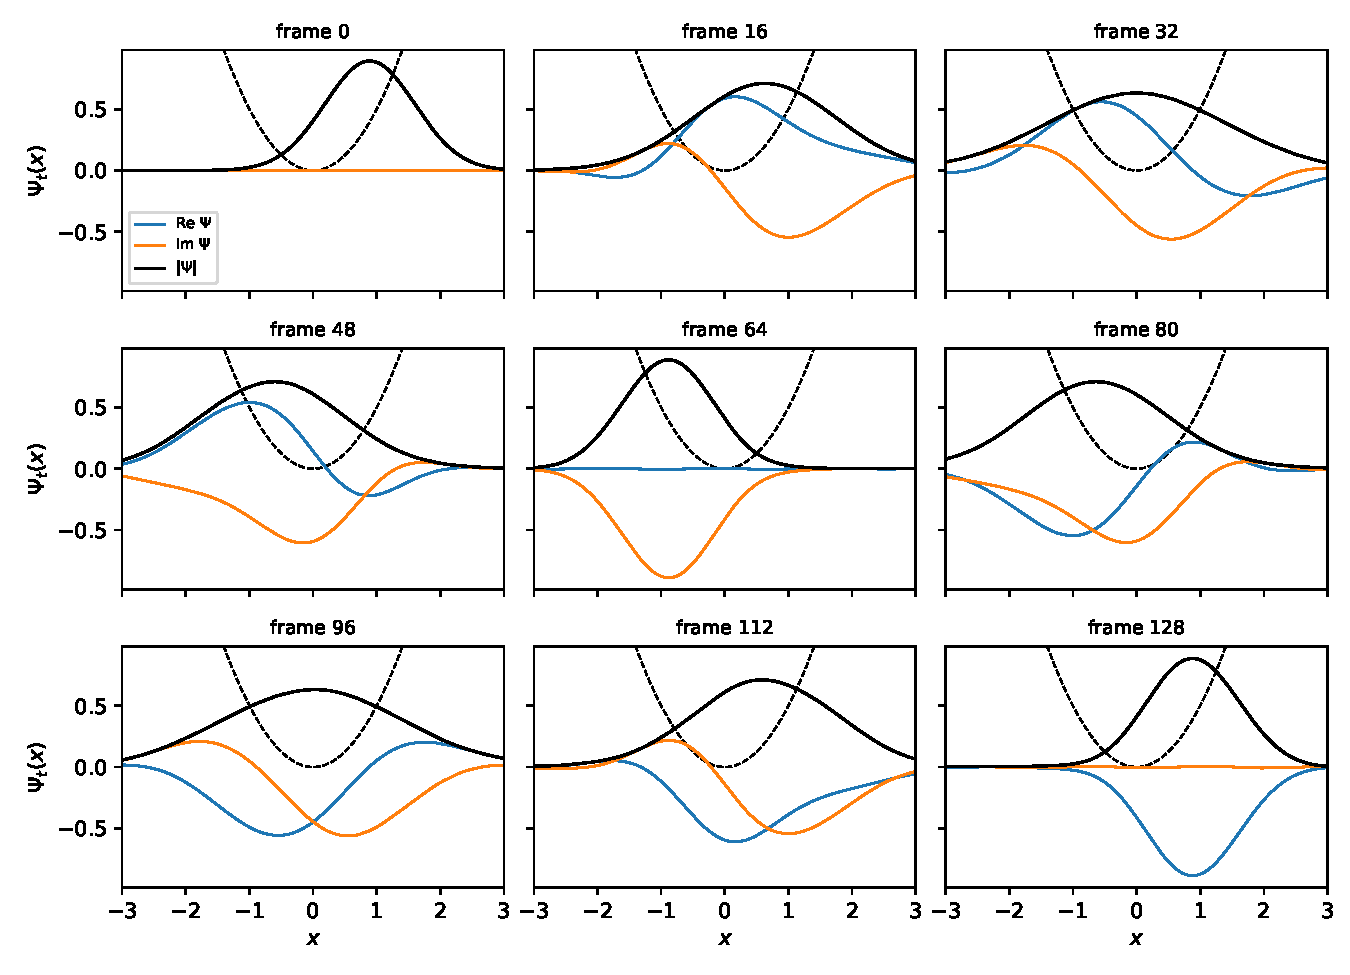
\includegraphics[width=0.85\textwidth]{figs/anim_frames.pdf}
  \caption{Frames $0,16,\dots,128$ of \texttt{animation.gif}. After one full period, $|\Psi|$ returns to its initial shape and $\Psi(T_0)=-\Psi_0$, since $e^{-iHT_0}=e^{-2\pi i(n+1/2)}=-1$ for every eigenstate.}
\end{figure}

%--------------------------------------------------------------------
\section*{Problem F (bonus): norm without renormalization}
\paragraph{Prediction (made before running).}
The phase of $K_\epsilon$ is $\phi=[(x_a^2+x_b^2)\cos\epsilon-2x_ax_b]/(2\sin\epsilon)$. As a function of $x_a$ it oscillates with local wavenumber
\[
  k(x_a,x_b)=\left|\frac{\partial\phi}{\partial x_a}\right|=\frac{|x_a\cos\epsilon-x_b|}{\sin\epsilon}\;\lesssim\;\frac{8}{\sin\epsilon}\quad\text{on }[-4,4].
\]
The sum over $x_a$ can only represent the integral if $\Delta x$ resolves these oscillations.
A Nyquist-type estimate (phase step $k\Delta x<\pi$) gives $8\Delta x/\sin\epsilon\approx0.28$ for (i), $8.7$ for (ii), and $8.7$ for (iii).
So I predicted that \textbf{(ii) and (iii) fail and (i) works}. The main run ($\epsilon=T_0/128$, $N_D=600$) gives $2.2$ and is fine.
Note the counterintuitive direction: a \emph{smaller} time step makes things worse, because $K_\epsilon$ oscillates faster as $\epsilon\to0$, where it approaches a $\delta$-function.

\begin{figure}[H]
  \centering
  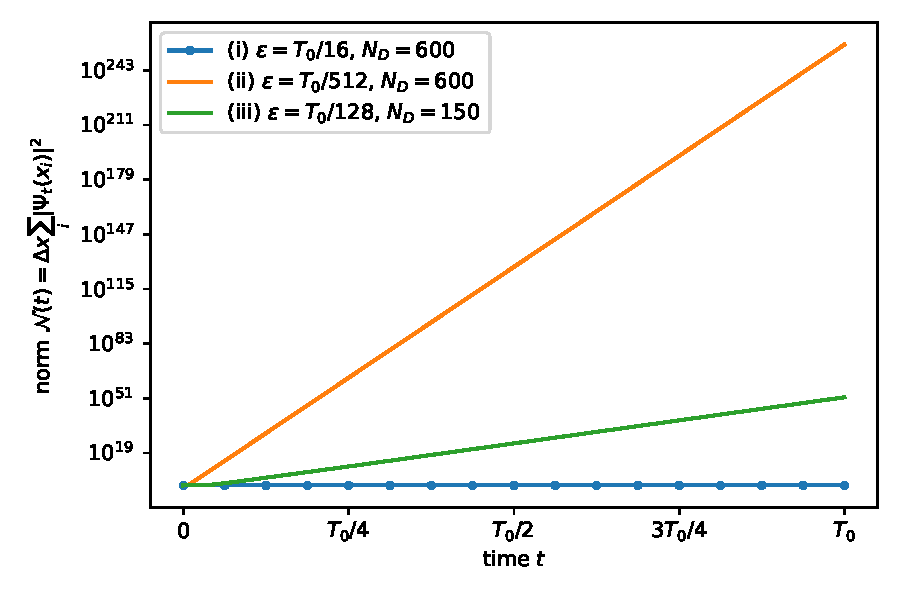
\includegraphics[width=0.49\textwidth]{figs/norm.pdf}\hfill
  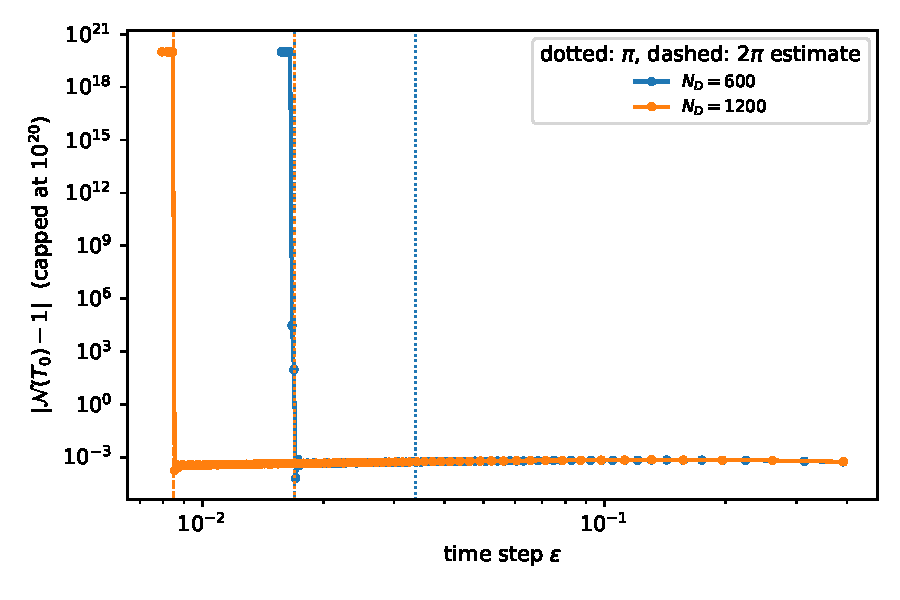
\includegraphics[width=0.49\textwidth]{figs/norm_scan.pdf}
  \caption{Left: $\mathcal N(t)$ for the three cases (log scale). Right: $|\mathcal N(T_0)-1|$ after one period vs.\ $\epsilon=T_0/n$, for $N_D=600$ and $1200$. Dotted lines: phase step $\pi$ per $\Delta x$. Dashed lines: phase step $2\pi$ per $\Delta x$. Values are capped at $10^{20}$ for plotting.}
\end{figure}

\paragraph{Results.}
The prediction holds.
\begin{itemize}
  \item Case (i) stays at $\mathcal N(T_0)=\normI$; the only loss is the wall leakage from Problem B.
  \item Case (ii) reaches $\mathcal N(T_0)=\normII$.
  \item Case (iii) reaches $\mathcal N(T_0)=\normIII$.
\end{itemize}
The two failing runs grow geometrically: a straight line on the log plot, by a factor $\approx3.2$ and $\approx2.5$ per step.
Once the kernel is undersampled, $\Delta x\,K_\epsilon$ is no longer a unitary matrix. Repeated application then amplifies its eigenvector with $|\lambda|>1$ exponentially.

\paragraph{Explanation and smallest time step.}
The $\pi$ criterion turns out to be conservative by a factor of 2.
Poisson summation explains why: $\Delta x\sum_jf(x_j)=\sum_m\int f(x)\,e^{2\pi imx/\Delta x}\,dx$.
For $f=K_\epsilon\Psi$, the alias terms ($m\neq0$) oscillate rapidly and cancel, unless they have a stationary point. That happens when $k$ reaches $2\pi/\Delta x$ somewhere on the grid.
The condition for the method to work is therefore
\[
  \frac{8\,\Delta x}{\sin\epsilon} < 2\pi
  \quad\Longrightarrow\quad
  \epsilon_{\min}\approx\frac{4\Delta x}{\pi}=\frac{32}{\pi N_D}.
\]
For $N_D=600$ this gives $\epsilon_{\min}\approx0.017\approx T_0/370$. The scan finds the first failure at $\epsilon=T_0/\nFailSix$.

Doubling $N_D$ halves $\Delta x$, which halves $\epsilon_{\min}$. The prediction is $T_0/740$ for $N_D=1200$, and the scan finds $T_0/\nFailTwelve$.
In other words, a finer time step must be paired with a proportionally finer grid: $\epsilon_{\min}\propto\Delta x\propto 1/N_D$.
There is no lower limit on $\epsilon$ from accuracy, since $K_\epsilon$ is exact for any $\epsilon$. The only approximation is the discretization of $x$.

%--------------------------------------------------------------------
\section*{AI use appendix}
\textcolor{red}{[To be written.]}

\end{document}
